\lecture{3. They Shall Be My People}{03}

\section*{Introduction}

\begin{frame}
\frametitle{Intro Story}
	\begin{center}
	pic something here
	\end{center}
\note{09:30}
\end{frame}

\begin{frame}
\frametitle{God wants a relationship with people}
\framesubtitle{Jeremiah 31:31-34}
	\keyversehiglight{they shall be my people}

\note{09:32}
\end{frame}

\begin{goals}
\goal Recognize that God wants a people who choose Him voluntarily
\goal Understand that God always provides for people to come to Him
\goal Appreciate how unique and special a Christian's relationship with God is

\note{09:33}
\note[item]{Some tough passages today.}
\end{goals}

\section{God wants volunteers}

\begin{frame}
\frametitle{The Israelites refused the Lord's feast}
\framesubtitle{Matt 22:1-14}

\note{09:35}
\note[item]{People don't love the Lord}
\note[item]{He's offering them something for the feast.  All they have to do is show up.}
\end{frame}

\begin{frame}
\frametitle{Even those who are following can eventually be rejected}
\framesubtitle{Matt 22:1-14}

\note{09:35}
\note[item]{There's a consequence for not following}
\note[item]{Matt. 7:21 Not everyone who says to me Lord, Lord will enter the kingdom of heaven but he who does the will of my father.}
\end{frame}

\begin{frame}
\frametitle{Many are called few are chosen.}
\framesubtitle{Matt 22:1-14}

\note{09:35}
\note[item]{God's people will be special because He chose them, but also because they chose Him.}
\end{frame}

\begin{frame}
\frametitle{Another volunteers slide}

\note{09:38}
\end{frame}

\section{God makes a way}

\begin{frame}
\frametitle{God will resurrect his people}
\framesubtitle{Ezekiel 37:7-10}
\begin{center}
	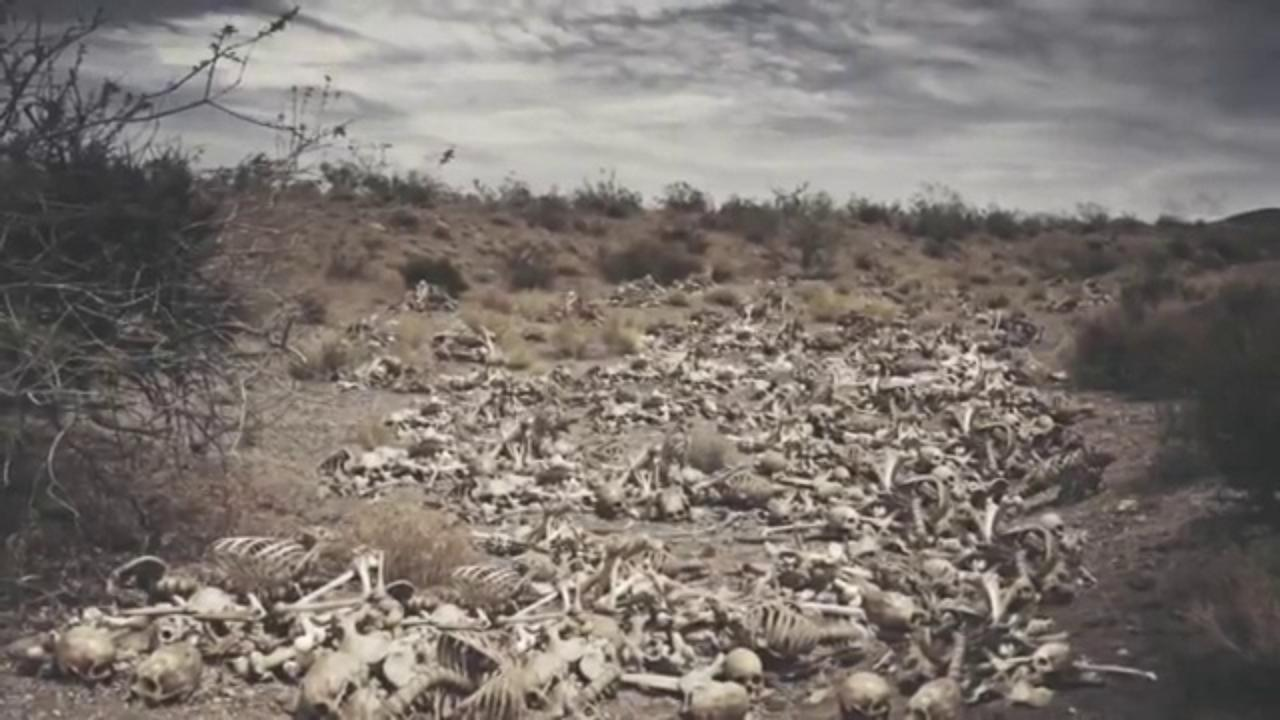
\includegraphics[width=\columnwidth]{figures/valleyOfDryBones.jpg}
\note{09:40}
\note[item]{Vs. 11 says explicitly that the bones are the whole house of Israel.
\note[item]{Says God will put His Spirit within them}
\note[item]{Land must be figurative.  This is premellinalism.}
\note[item]{They will no longer be a divided kingdom.  But, Ezekiel was prophesying during captivity after Israel had already been taken away.}
\note[item]{Clearly this has to be Christians.}
\end{center}

\note{09:40}
\note[item]{The dead shall live and you shall know that I am the Lord}
\note[item]{Resurrection is a key feature of the people of God.}
\end{frame}

\begin{frame}
\frametitle{God adopts us as sons}
\framesubtitle{Romans 8:12-17}

\note{09:41}
\end{frame}

\section{You are special}

\begin{frame}
\frametitle{The Lord set aside Israel}
\framesubtitle{Deut. 10:12-22}

\note{09:48}
\end{frame}

\begin{frame}
	\frametitle{The Lord predestined his type of people}
	\framesubtitle{Romans 8:28-30}
	
	\note{09:50}
	\note[item]{Where Calvinists get it wrong is misunderstanding the sovereignty of God.}
	\note[item]{I, personally, have no issue with God knowing what happens in the future or even knowing ahead of time the names of those who will be saved.}
	\note[item]{He certainly knew ahead of time the poor decisions people would make, (Rom 9, Esau and Pharaoh, Judas, Peter, etc.).}
	\note[item]{And, a truly all-powerful God has the power to make things work in His way and in His time without forcing people to do things.}
	\note[item]{What I have a problem with is that God `selected' people apart from the decisions they make.}
	\note[item]{Calvinists assume that man is fallen from birth, and thus the decisions we make are \emph{totally} determined by either our sinful human nature (over which we have no control) or the miraculous influence of the Holy Spirit (for salvation).}
	\note[item]{This is basically the same problem that sociologists have.  The whole field of sociology is predicated on the assumption that your environment (family, culture, socioeconomic status) and to some extent your genetics are the sole determinants of your choices you make.  
	\note[item]{This is simply counter to the Bible.}
	
\end{frame}

\begin{frame}
	\frametitle{The Lord's people are a chosen race and royal priesthood}
	\framesubtitle{I Peter 2:9-10}
	\note{09:53}
	\note[item]{	}
\end{frame}

\section{Review}

\begin{frame}
\frametitle{They shall be my people}
	\begin{itemize}
		\item God wants volunteers
		\item God makes a way
		\item You are special
	\end{itemize}
\note{10:10}
\note[item]{Are you proud of being on God's team?}
\end{frame}